\documentclass[a4paper,10pt]{report}
\usepackage[utf8]{inputenc}
\usepackage{amsmath}
\usepackage{amssymb,amsfonts,textcomp}
\usepackage{array}
\usepackage{hhline}
\usepackage{hyperref}
\hypersetup{colorlinks=true, linkcolor=blue, citecolor=blue, filecolor=blue, urlcolor=blue, pdftitle=, pdfauthor=Gilles Vuidel, pdfsubject=, pdfkeywords=}
\usepackage{graphicx}
\usepackage[top=2.5cm,bottom=2.5cm,left=2.5cm,right=2.5cm,nohead]{geometry}
\usepackage{float}
\usepackage{parskip}
\usepackage{multirow}
\usepackage{caption}
\usepackage{fancyvrb}
\makeatletter
\newcommand\arraybslash{\let\\\@arraycr}
\makeatother
% centering figures
\makeatletter
\g@addto@macro\@floatboxreset\centering
\makeatother
\setlength\tabcolsep{1mm}
\renewcommand\arraystretch{1.3}

% saut après itemize
\let\EndItemize\enditemize
\def\enditemize{\EndItemize\medskip}


\begin{document}
\begin{titlepage}
	
	\centering
	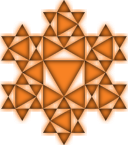
\includegraphics[scale=0.5]{img/logo.png}\\
	
	\bigskip
	\bigskip
	\bigskip	
	{\Huge
		\bfseries
		Fractalyse 3.0 (FracGIS)\\
		\bigskip
		User manual\\
	}
	\bigskip
	\bigskip
	\bigskip
	\bigskip
	\bigskip
	
	{\Large		
		Gilles Vuidel, Cécile Tannier and Pierre Frankhauser\\
		\bigskip
		2016-09-13\\
	}
	
\end{titlepage}

\parindent 0pt

\tableofcontents

\chapter{Introduction}
\section{About Fractalyse 3.0}
Fractalyse is a software application for analysing 2D texture by fractal theory. 
The version 3 of Fractalyse has been completely rewritten in Java language, to improve data management with GIS (Geographical Information System) support, graphical user interface and performance with parallelism. It runs on any computer supporting Java Virtual Machine.
\section{Authors}
Fractalyse has been developed by Gilles Vuidel, Cécile Tannier and Pierre Frankhauser at ThéMA laboratory (University of Franche-Comté – CNRS). 
\section{Terms of use}
Fractalyse is distributed free-of-charge. Users must cite the following reference in their publications:
????
The source code is available and licensed in GPLv3.
\section{System requirements}
Fractalyse 3.0 runs on any computer supporting Java 1.7 or later (PC under Linux, Windows, Mac, etc.). However,
when dealing with very large datasets, the amount of RAM memory in the computer will limit the maximum image size that can be processed in a single run with Fractalyse. In addition, for some methods, processing power (CPU) will determine the speed of computing. For details, see section 8 below.
\section{Installing the software}
Fractalyse can be downloaded from http://www.fractalyse.org

Download and install Java 1.7+ from java.com. If you have a 64-bit operating system, it is best to install the 64-bit version of Java.
Download fractalyse-3.0.jar and launch it.


\part{Graphical interface}

\chapter{Data}
Fractalyse can read 2 types of data : vector and raster.
\section{Loading data : File menu}
\subsection{Vector format}
Shapefile format is a vector GIS file format created by ESRI for its GIS ArcGIS.
This format supports 3 type of geometry : point, linestring and polygon.
Fractalyse support all these types. 
\subsection{Raster format}
Fractalyse support 2 raster format : TIFF and Ascii Grid.

Ascii grid is a text format. The image is written as a matrix preceded by a header of 5 lines :
\begin{Verbatim}
	ncols	5
	nrows	5
	xllcorner	0
	yllcorner	0
	cellsize	1
	1 0 0 0 1
	0 1 0 1 0
	0 0 1 0 0
	0 1 0 1 0
	1 0 0 0 1
\end{Verbatim}

TIFF is a binary format commonly used for raster image. It can contains an extension named GeoTIFF, which added spatial references to the image. Fractalyse can load TIFF image with or without GeoTIFF extension. Fractalyse does not support RVB color image.

When the image file is loaded with the menu "Load raster data", a new layer is created and the image is displayed. If the image contains only 0 and 1 value, Fractalyse set the layer as binary layer and set white color for 0 and black color for 1. Otherwise, it sets a gray scale color ramp for the image.


\section{Data manipulation : Tools menu}
For some analyses the vector data type is not supported for example correlation) and for raster data type, most analyses need binary image. Fractalyse contains some functions in Tools menu to convert vector to raster data (Rasterize menu) and to convert grayscale raster to binary (Binarize menu).
\subsection{Rasterize menu : convert vector to raster}

\subsection{Binarize menu}
\subsection{Negative menu}
\subsection{Selection menu}

\chapter{Fractal analysis}
\section{Vector menu}

\section{Raster menu}

\section{Network menu}

\chapter{Miscellaneous}
\section{Preferences menu}
\subsection{Memory}

\subsection{Processors}

\section{Log window}



\part{Command line interface}

\chapter{Prerequisite}

Fractalyse can be used in command line interface (CLI).
It is useful for executing Fractalyse on a distant computer without a graphical interface, or batching some processes that are not available in the graphical user interface (GUI).

\section{Launch Fractalyse in CLI mode}
First you have to open a terminal window.
Then, go to the directory of the Fractalyse program with \textit{cd} command.
Finally, type the following command to display the Fractalyse help screen :
\begin{Verbatim}
java -jar fractalyse-3.0.jar --help
\end{Verbatim}
Result
\begin{Verbatim}
Usage :
java -jar fractalyse.jar [-proc n]
...
...
\end{Verbatim}
You're ready to use Fractalyse in CLI mode !

\section{Syntax}
\subsection{Definition}
Commands always start with a double dash.\\
A global option starts with only one dash.\\
A parameter does not have a dash.\\
\subsection{Character separator}
Blank spaces are used to separate commands and parameters. You cannot have a name containing blank spaces.\\

\subsection{Optional parameter}
Parameters enclosed in brackets are optional. 
Therefore, parameters not in brackets are mandatory.


\subsection{Command execution}
Fractalyse can execute only one command.

\begin{Verbatim}
java -jar fractalyse-3.0.jar ...
\end{Verbatim}




\chapter{Command reference}
\section{General command}
\subsection{--help : display help}
Command :

\begin{Verbatim}
	java -jar fractalyse-3.0.jar --help
\end{Verbatim}

Result :
\begin{Verbatim}
Usage :

\end{Verbatim}


\section{Options}

\subsection{-proc}
Defines the number of processors (or cores) used by Fractalyse.
By default, CLI mode uses the value defined in the preferences window.
See the parallelism section for more details.


\chapter{Command examples}




\chapter{Performance tuning}
\section{Parallelism to speed up execution}
\subsection{One computer : threads}
If your computer has more than one core (most of them), you can take advantage of parallelism. 
Most Fractalyse commands are parallelized. You can speed up command execution by defining the number
of cores (or processors) used by Fractalyse with the option \textit{-proc} after the project command :
\begin{Verbatim}
java -jar fractalyse-3.0.jar -proc 8 ...
\end{Verbatim}
By default, CLI mode uses the number of processors defined in the preferences window of the GUI.
\subsection{Computer cluster : mpi}
Fractalyse can be run on computer clusters wich support Java for OpenMPI.
\begin{Verbatim}
mpirun java -jar fractalyse-3.0.jar --mpi  ...
\end{Verbatim}
Only some commands can be used in mpi environments : --gmetric, --cmetric, --lmetric, --delta, --addpatch
\section{Memory management}
In CLI mode, the memory configuration defined in the preferences window cannot be used.
By default, the amount of memory available for Fractalyse is system dependent. It can vary from 128 Mb to several Gb.
In most cases, Fractalyse will run normally. But if you have a large image, some commands would be slow or even crash due to memory limitation.
If Fractalyse execution terminates with OutOfMemoryError, GC overhead or Java Heap space, you need to increase memory allocated to Fractalyse.

To define manually the maximum amount of memory allocated to Fractalyse, use Java option -Xmx :
\begin{Verbatim}
java -Xmx2g -jar fractalyse-3.0.jar ... # 2Gb allocated
java -Xmx1500m -jar fractalyse-3.0.jar ... # 1500 Mb -> 1.5Gb allocated
\end{Verbatim}
If you cannot allocate more than 1Gb or 1.5G and your computer has more memory available, you have probably a
 32-bit version of Java, which is limited to less than 2Gb of memory.
Check your Java version :
\begin{Verbatim}
java -version
\end{Verbatim}
If it is a 32-bit version, install a 64-bit Java version to handle all your computer memory.

\end{document}          
